\chapter{\emph{Advanced Encryption Standard} (AES)}
\section{Storia}
\paragraph{Nuovo bando} Nel giugno 1998 esce il bando organizzato dal NIST per individuare un nuovo algoritmo in grado di soppiantare il DES ed il 3DES. Le proposte dovevano tenere conto dei seguenti elementi:
\begin{itemize}
    \item \textbf{sicurezza}: resistere a tutti gli attacchi noti 
    \item \textbf{costo di realizzazione}: doveva essere facile implementarlo sia in software che in hardware 
    \item \textbf{libero da brevetti} in quanto il nuovo standard doveva divenire libero da utilizzare 
    \item \textbf{caratteristiche algoritmiche}: portabile su diverse macchine, usabile con chiavi di diversa lunghezza [Novità!]
\end{itemize}
Ci furono 21 proposte. Già nell'agosto 1998 furono scartati 6 cifrari, e nell'aprile 1999 ne rimasero solo 5.

\paragraph{Sfida finale} I cifrari arrivati alla fine furono:
\begin{itemize}
    \item MARS (IBM)
    \item RC6 (RSA)
    \item \textbf{\underline{Rijndael}} (Proton word int + Università di Leuven, Belgio)
    \item SERPENT (Università di Israele, UK, USA)
    \item TWOFISH (Berkeley, Princeton)
\end{itemize}

\paragraph{Scelta definitiva} In ottobre 2000 Rijndael vinse il bando e diventò AES con qualche modifica.  Nel 2001 AES diventa ufficialmente lo standard. E' un algoritmo che ancora oggi continua a conservare tutti i bit di sicurezza.

\section{Caratteristiche}
\subsection{Dimensione della chiave e numero di fasi} L'AES accetta chiavi da 128, 192, 256 bit. Noi vedremo la versione a 128 bit (ancora oggi tutti bit di sicurezza). E' anch'esso un cifrario a fasi (come il DES), dove il numero di fasi dipende dal numero di bit della chiave:
\begin{itemize}
	\item 10 fasi $\xrightarrow{}$ 128 bit
	\item 12 fasi $\xrightarrow{}$ 192 bit
	\item 14 fasi $\xrightarrow{}$ 256 bit
\end{itemize}

\subsection{Preparazione: selezione della sottochiave di ogni fase}
\[\boxed{\text{Possibile scegliere in anticipo tutte le chiavi.}}\]
La prima differenza rispetto al DES è il processo di selezione delle sottochiavi di fase. Ogni fase utilizza 128 bit di chiave, a partire da questa calcoliamo nuove chiavi attraverso un processo deterministico. Collochiamo la nostra chiave in una matrice $4 \times 4$ (ogni elemento contiene 8 bit, 32 bit per colonna):
$$
K = 
    \begin{bmatrix}
        K[0] & K[4] & K[8] & K[12] \\
        K[1] & K[5] & K[9] & K[13] \\
        K[2] & K[6] & K[10] & K[14] \\
        K[3] & K[7] & K[11] & K[15]
    \end{bmatrix}
$$
\noindent Nelle dieci fase successive diamo in input nuove matrici $K$. La cosa nuova è che il procedimento utilizzato nelle fasi per ricavare le chiavi non è lineare (come invece è nel DES). 
\paragraph{Procedimento} Prese le colonne in ordine da sinistra verso destra abbiamo: 
$$W(0), W(1), W(2), W(3)$$
Costruiamo quindi $W(i)$ che è una sequenza di byte che usiamo per generale le sottochiavi di fase.
Per ogni $t \geq 4$ otteniamo
\[
    W(t) = 
    \begin{cases}
        W(t-1) \oplus W(t-4) \text{ se t non è multiplo di 4} \\
        T(W(t-1)) \oplus W(t-4) \text{ se t è multiplo di 4}
    \end{cases}
\]
T è una funzione non lineare applicata tramite una S-box.
\paragraph{Chiave dell'$i$-esima fase} La chiave dell'$i$-esima fase è quindi composta da:
$$W(4 \cdot i), W(4 \cdot i + 1), W(4 \cdot i + 2), W(4 \cdot i + 3)$$
Complessivamente abbiamo fatto un'\textbf{\underline{espansione non lineare}} da 4 colonne a 44 colonne. Le chiavi per tutte le fasi sono pronte.

\subsection{Preparazione: cifratura per blocchi}
La cifratura si fa per blocchi (di 128 bit in questo caso).
Si creano i blocchi caricandoli \emph{per colonna} in una matrice $4 \times 4$ (anche in questo caso abbiamo 1 byte in ogni elemento):
$$
B = 
    \begin{bmatrix}
        b_{00} & b_{01} & b_{02} & b_{03} \\
        b_{10} & b_{11} & b_{12} & b_{13} \\
        b_{20} & b_{21} & b_{22} & b_{23} \\
        b_{30} & b_{31} & b_{32} & b_{33}
    \end{bmatrix}
    \,\,\,\,\,b_{ij} \in \{0, 1\}^{8}
$$
\paragraph{Prima trasformazione} Si applica una prima trasformazione applicando la chiave:
$$ B \longrightarrow B \oplus K $$

\subsection{Fasi}
\begin{framed}
	\noindent \textbf{Domanda da esame}. Descrivere il cifrario AES, e in particolare le quattro operazioni eseguite in ciascuna fase.
\end{framed} 
Dopodiché si inizia con le fasi, ognuna di esse composta da 4 operazioni:
\begin{itemize}
    \item \emph{substitute bytes} (applicazione della S-box)
    \item \emph{shift rows} (dipendenza degli elementi di una colonna dagli elementi delle altre colonne)
    \item \emph{mix columns} (non si applica nella decima fase, dipendenza dell'elemento di una colonna dagli altri elementi della colonna)
    \item \emph{add round key} (applicazione della chiave $i$-esima)
\end{itemize}
Le prime 3 operazioni applicano: non linearità, diffusione e confusione. L'ultima fase aggiunge la chiave. Alla fine delle iterazioni si ottiene il crittogramma.
La S-Box dell'AES è sempre usata in forma di tabella di verità, ma a differenza di quella del DES si conosce la funzione che la genera!

\subsubsection{\emph{Substitute bytes} (S-box)}
Ogni byte viene trasformato usando la S-Box:
$$ b_{ij} \xrightarrow{} \text{S-Box}(b_{ij}) $$
La S-Box è diversa rispetto a quella del DES, dove la S-box è stata imposta in sola forma tabellare (\textbf{\underline{uno degli aspetti più criticati del DES}}, principalmente per sospetti di \emph{trapdoor}). Questa S-Box è presentata in forma tabellare, ma si conosce in modo chiaro le operazioni algebriche eseguite: si compone di una matrice $16 \times 16$ di interi $\in [0, 255]$ e contiene una permutazione dei numeri di questo intervallo.
L'accesso alla S-Box viene fatto suddividendo il byte $b_{ij}$ in due blocchi da 4 bit l'uno:
$$ b_{ij} = b_{1}b_{2}b_{3}b_{4} \mid b_{5}b_{6}b_{7}b_{8} $$
i primi 4 bit formano il numero di \emph{riga} ($0 \leq x \leq 15$), gli ultimi 4 bit formano il numero di \emph{colonna} ($0 \leq y \leq 15$).
\paragraph{Esempio} Prendiamo
$$ b_{ij} = 10001011 $$
spezziamo a metà: $1000$ è $8$, mentre $1011$ è 11. Nella tabella che definisce la S-box otterremo
$$\text{S-box}[8,11]=61=(00111101)_2$$
\paragraph{Relazione algebrica implementata} La relazione implementata dalla S-Box è:
$$ x \xrightarrow{} x^{-1} + c $$
questo inverso è l'\textit{inverso moltiplicativo del byte} (spiegato più avanti nelle nozioni di Algebra lineare) calcolato nel campo $\text{GF}(2^{8})$ (\textit{Campo di Galois}, campo finito) con l'aggiunta di una componente lineare. In questo insieme:
\begin{itemize}
	\item la somma viene eseguita tramite lo XOR (somma modulo 8)
	\item la moltiplicazione è eseguita $\text{mod } 2^{8}$.
\end{itemize}
Nella pratica ogni byte può essere visto come un polinomio, facendo la moltiplicazione si fa il prodotto tra polinomi ma in modulo, quindi si tagliano via i gradi oltre al settimo. 
\paragraph{Miglioramento} Questa S-Box ha una bassissima correlazione tra i bit di ingresso e di uscita. Inoltre essendo usata sia per la chiave che per la matrice del messaggio si ha una maggiore sicurezza



\subsubsection{\emph{Shift rows} (Diffusione)}
Si usa per spargere il messaggio.
Lascia invariata la prima riga, shifta a sx le altre righe, rispettivamente di 1, 2 e 3 posizioni.
$$
    \begin{bmatrix}
        b_{00} & b_{01} & b_{02} & b_{03} \\
        b_{10} & b_{11} & b_{12} & b_{13} \\
        b_{20} & b_{21} & b_{22} & b_{23} \\
        b_{30} & b_{31} & b_{32} & b_{33}
    \end{bmatrix}
\xrightarrow{}
    \begin{bmatrix}
        b_{00} & b_{01} & b_{02} & b_{03} \\
        b_{11} & b_{12} & b_{13} & \mathbf{b_{10}} \\
         b_{22} & b_{23} & \mathbf{b_{20}} & \mathbf{b_{21}} \\
        b_{33} & \mathbf{b_{30}} & \mathbf{b_{31}} & \mathbf{b_{32}}
    \end{bmatrix}
$$
Ho quindi diffuso i byte di ogni colonna su tutte le altre.

\subsubsection{\emph{Mix columns} (Diffusione)}
Si prende ogni colonna della matrice, viste come vettori, e si moltiplicano per una matrice. Abbiamo una matrice $M$ di dimensione $4 \times 4$ byte, per ogni colonna:
$$
    B_{j} \xrightarrow{} M \cdot B_{j}
$$
con $0 \leq j \leq 3$. Anche qui si lavora in GF($2^8$). \textbf{Questo porta ogni elemento della colonna ad essere dipendente da tutti i byte della colonna}. La matrice $M$ è pensata in modo tale che ogni byte di una colonna influenzi tutti i byte della stessa colonna.
$$b_{ij} \text{ dipende da tutti i byte: $b_{0j}, b_{1j}, b_{2j}, b_{3j}$}$$

\subsubsection{\emph{Add round key} (Confusione)}
Facciamo somma della chiave di base, poco da dire:
$$
    b_{ij} \xrightarrow{} b_{ij} \oplus K_{ij} \text{ chiave della sottofase}
$$


\subsection{\emph{Cipher Block Chaining} (CBC)}
Sia il DES che l'AES cifrano il \textit{plaintext} a blocchi, AES ad esempio divide in blocchi grandi quanto la chiave e poi si cripta. Il problema di ciò è che blocchi uguali vengono cifrati allo stesso modo (si usa sempre la stessa chiave in una sessione), questo può dare molte informazioni al crittoanalista.
\paragraph{Soluzione} Per risolvere questo problema si stabilisce una dipendenza tra blocco $i$-esimo e precedenti. Nell'AES si prende il messaggio $m$ e lo si divide in blocchi da 128 bit:
$$ m = m_{1}m_{2}\dots m_{i} \dots m_{e} $$
\begin{itemize}
    \item se $\mid m_e \mid < 128$ allora si aggiunge una sequenza $10...0$ fino ad arrivare a 128 bit;
    \item se invece $| m_e | = 128 $ si inserisce comunque un intero blocco $10...0$ in modo da avere sempre questo terminatore.
\end{itemize}
Successivamente si sceglie una sequenza iniziale $c_0$ random, che può anche essere trasmessa in chiaro, e si attua questo schema:
\begin{center}
    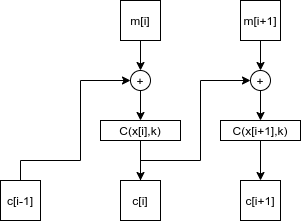
\includegraphics[width = 170pt]{images/CBC.png}
\end{center}
\begin{align*}
	x_{i} = m_{i} \oplus c_{i-1} && c_{i} = C(m_{i} \oplus c_{i-1}, K)
\end{align*}
\noindent questa modalità è detta \emph{Cipher Block Chaining} (CBC).
\paragraph{Decifrazione} La decifrazione invece si esegue in questo modo:
\begin{center}
    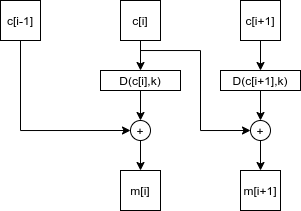
\includegraphics[width = 170pt]{images/CBC_2.png}
\end{center}
$$
    m_i = D(c_i, K) \oplus c_{i-1}
$$
\paragraph{Osservazione} Mentre la cifratura va eseguita necessariamente sequenzialmente (visto che un elemento dipende dal precedente) la decifratura si può eseguire in parallelo (abbiamo tutti gli elementi, non dobbiamo attendere il precedente).
Inoltre se invio il testo cifrato e ci sono errori risulta in un errata decifrazione solo del blocco $i$ e $i+1$ mentre gli altri continuano ad essere decriptati correttamente.
